\documentclass{article}
\usepackage{amsmath,amsfonts,fancyhdr,parskip,amssymb,graphicx}
\usepackage[margin = 1.5in]{geometry}
\pagestyle{fancy}
\lhead{Ben Carriel (bkc39)}
\chead{Bryan Cuccioli (blc72)}
\rhead{Andy Levine (awl58)}
\setlength{\parindent}{1cm}

\DeclareMathOperator{\oh}{\mathcal{O}}
\DeclareMathOperator{\ta}{\xrightarrow{\ \ \ }}
\DeclareMathOperator{\opt}{\texttt{OPT}}
\newcommand{\problem}[1]{\noindent {\bf #1}}

\begin{document}

\problem{Problem 1.} The counterexample is the following graph:

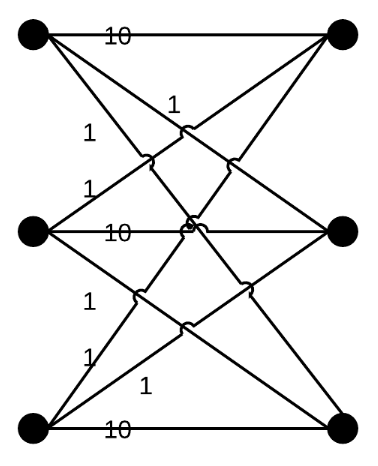
\includegraphics[width=50mm]{grapha.png}

\end{document}
